\documentclass[12pt,letterpaper]{article}

% ==================== PAQUETES ====================
\usepackage[spanish]{babel}
\usepackage{caption}
\usepackage{csquotes} 
\usepackage[style=apa]{biblatex}
\usepackage{fontspec}
\usepackage{microtype}
\usepackage{float}
\usepackage{graphicx}
\usepackage{indentfirst}
\usepackage{setspace}
\usepackage{hyperref}
\usepackage[margin=2.54cm]{geometry}
\usepackage{listings}
\usepackage{xcolor}
\usepackage{booktabs}
\usepackage{longtable}
\usepackage{enumitem}

% ==================== CONFIGURACIÓN GENERAL ====================
\setmainfont{Arimo}
\doublespacing
\renewcommand{\arraystretch}{1.35}
\addto\captionsspanish{\renewcommand{\tablename}{Tabla}}
\addbibresource{ref.bib}
\graphicspath{{images/}}

% ==================== LISTINGS (CÓDIGO) ====================
\lstset{
  basicstyle=\ttfamily\small,
  breaklines=true,
  frame=single,
  numbers=left,
  numberstyle=\tiny,
  keywordstyle=\color{blue},
  commentstyle=\color{green!60!black},
  stringstyle=\color{red},
  showstringspaces=false,
  language=bash
}

% ==================== HYPERREF ====================
\hypersetup{
  colorlinks=true,
  linkcolor=black,
  citecolor=black,
  urlcolor=blue,
  pdfauthor={Jorge Iván Acosta Aristizábal, [Compañero 1], [Compañero 2]},
  pdftitle={Automatización de la configuración de almacenamiento en máquinas virtuales GNU/Linux desde el host con Oracle VM VirtualBox},
  pdfsubject={Computación en la Nube - Parcial 1},
  pdfkeywords={VirtualBox, Guest Additions, automatización, almacenamiento, GNU/Linux, cloud computing}
}

% ==================== MACROS PERSONALIZADAS ====================
\newcommand{\vm}{\textit{VM}}
\newcommand{\host}{\textit{host}}
\newcommand{\guestadditions}{Guest Additions}

\begin{document}

% ==================== PORTADA ====================
\thispagestyle{empty}
\begin{center}
    \textbf{Automatización de la configuración de almacenamiento en máquinas virtuales GNU/Linux desde el host con Oracle VM VirtualBox}\\[2cm]

    \textbf{Estudiantes:}\\[0.5cm]
    Jorge Iván Acosta Aristizábal \\ [3.5cm]

    
\includegraphics[height=4cm]{logo.png}\\[3cm]

    \textbf{Universidad del Quindío} \\
    \textbf{Facultad Ingeniería} \\
    \textbf{Ingeniería de Sistemas y Computación} \\
    Computación en la Nube \\
    Armenia, Quindío\\
    Octubre del 2026
\end{center}

\newpage

% ==================== CUERPO ====================
\pagestyle{plain}
\tableofcontents
\newpage

% ==================== INTRODUCCIÓN (INLINE) ====================
\addcontentsline{toc}{section}{Introducción}

\noindent En prácticas previas de la asignatura se realizó manualmente la preparación de un disco adicional para ser utilizado como almacenamiento de datos en una máquina virtual GNU/Linux. Dicha actividad implicó ejecutar secuencialmente los procedimientos de particionado, creación del sistema de archivos (ext4/xfs), montaje y configuración del montaje automático mediante \texttt{/etc/fstab} para garantizar persistencia \parencite{linux_storage_management}. Si bien estos pasos son fundamentales para la administración de almacenamiento, su ejecución manual resulta repetitiva, propensa a errores humanos y no escala cuando una organización debe aprovisionar almacenamiento en múltiples máquinas virtuales.

El presente trabajo aborda la automatización completa de este proceso desde el sistema operativo \host{}, aprovechando las capacidades de Oracle VM VirtualBox. La solución permite que el \host{} inicie y prepare una \vm{}, establezca comunicación con el sistema operativo invitado mediante las \guestadditions{} y ejecute automáticamente las acciones necesarias para que el nuevo almacenamiento quede disponible sin intervención manual. Los requisitos fundamentales son la ejecución desatendida, sin ingreso de contraseñas, comandos interactivos ni pulsaciones de tecla; la reproducibilidad, con el mismo resultado en cada ejecución; la reutilización, aplicable a múltiples VMs con parámetros configurables; y la idempotencia, con re-ejecución segura sobre VMs ya configuradas sin pérdida de datos ni operaciones destructivas \parencite{idempotency_concept}.

La comunicación \host{}-\vm{} se realiza a través de la Guest Control API (\texttt{VBoxManage guestcontrol}), mecanismo nativo de VirtualBox que no requiere configuración de red adicional más allá del modo puente (\textit{bridged networking}) para la obtención de la IP de la \vm{} \parencite{virtualbox_guestcontrol, virtualbox_networking}. La automatización se implementa en Bash para \host{} Linux/macOS, siguiendo prácticas robustas de scripting \parencite{bash_best_practices, shellcheck} y validada con el framework de testing BATS \parencite{bats_testing}. De este modo, el aprovisionamiento deja de depender de pasos manuales y se convierte en un procedimiento desatendido y verificable, cuyos resultados son consistentes entre ejecuciones y cuya repetición no compromete al sistema invitado.



% ==================== CAPÍTULOS MODULARES ====================
% ==================== MARCO TEÓRICO Y TECNOLOGÍAS ====================
\section{Marco Teórico y Tecnologías}

La solución descrita en este documento se inscribe en la confluencia de tres áreas complementarias de la administración de sistemas. La virtualización permite ejecutar sistemas operativos completos como \vm{} aisladas sobre un mismo equipo físico y expone los recursos, como discos e interfaces de red, que el \host{} puede administrar de forma programática \parencite{virtualbox_vboxmanage, virtualbox_networking}. La administración de almacenamiento en GNU/Linux, por su parte, define el procedimiento que se busca automatizar: dejar un disco disponible y persistente en el sistema invitado \parencite{linux_storage_management}. Por último, la automatización mediante scripts convierte ese procedimiento manual en una operación programada, reproducible e idempotente, es decir, capaz de repetirse sin alterar el resultado ni comprometer los datos ya existentes \parencite{idempotency_concept}. Estos tres frentes convergen cuando una organización debe preparar almacenamiento en múltiples \vm{} sin intervención manual, que es precisamente el escenario abordado a continuación.

\subsection{Virtualización y Oracle VM VirtualBox}

Oracle VM VirtualBox es un hipervisor de tipo 2 (alojado, \textit{hosted}), es decir, una aplicación que se instala sobre el sistema operativo del \host{} y permite ejecutar múltiples sistemas invitados como \vm{} independientes sin requerir modificaciones al sistema anfitrión \parencite{virtualbox_vboxmanage}. Este modelo resulta apropiado para entornos de trabajo y educativos, donde la instalación sencilla y la gestión centralizada desde una única interfaz son requisitos frecuentes.

Entre las capacidades de VirtualBox relevantes para este trabajo se encuentran la gestión de discos virtuales en formatos como \texttt{.vdi} y \texttt{.vmdk}, que permiten adjuntar almacenamiento adicional a una \vm{} sin intervención sobre hardware físico, y la configuración de red en modo puente (\textit{bridged networking}), en la cual la interfaz de la \vm{} se asocia a una interfaz física del \host{} y obtiene una dirección IP propia dentro de la red local \parencite{virtualbox_networking}. Asimismo, VirtualBox expone una interfaz completa de línea de comandos, \texttt{VBoxManage}, mediante la cual es posible crear, iniciar, detener y consultar \vm{}, administrar discos y snapshots y consultar o modificar propiedades; dicho comando constituye el punto de entrada para toda la automatización descrita en este documento \parencite{virtualbox_vboxmanage}.

\subsection{Guest Additions}

Las \guestadditions{} son un conjunto de controladores de dispositivo y servicios que se instalan dentro del sistema operativo invitado y que mejoran la integración y el rendimiento entre el \host{} y la \vm{}: gráficos acelerados, portapapeles compartido, redimensionamiento dinámico de la ventana y sincronización de hora, entre otros \parencite{virtualbox_guestadditions}.

Su componente de mayor relevancia para este trabajo es el servicio de Guest Control, que habilita desde el \host{} el comando \texttt{VBoxManage guestcontrol}. A través de este mecanismo es posible ejecutar programas en el invitado, copiar archivos, crear directorios y gestionar sesiones, autenticándose con un usuario y contraseña del propio sistema invitado \parencite{virtualbox_guestcontrol, virtualbox_advanced_topics}. Para que todo ello funcione, las \guestadditions{} deben estar instaladas en la \vm{} y el servicio \texttt{VBoxService} debe encontrarse en ejecución; de ello depende la ejecución desatendida que la solución propone \parencite{virtualbox_guestadditions}.

\subsection{Comunicación Host--Guest}

Existen varios mecanismos para ejecutar comandos en el invitado desde el \host{}, cada uno con un distinto nivel de dependencia respecto de la configuración de red.

La Guest Control API (\texttt{VBoxManage guestcontrol}) permite ejecutar procesos, transferir archivos y crear directorios dentro de la \vm{} sin que el invitado exponga servicios de red adicionales, pues la comunicación la transporta el propio hipervisor por medio de las \guestadditions{} \parencite{virtualbox_guestcontrol, virtualbox_advanced_topics}. Como alternativa, SSH con autenticación por clave ofrece un canal estandarizado y ampliamente disponible en sistemas GNU/Linux, siempre que la \vm{} ejecute un servidor SSH y exista conectividad de red; su configuración comprende el intercambio de llaves y opciones de cliente como \texttt{StrictHostKeyChecking}, \texttt{UserKnownHostsFile} y \texttt{ConnectTimeout} \parencite{ssh_key_auth, ssh_config}. Finalmente, las carpetas compartidas facilitan la transferencia de archivos entre \host{} y \vm{}, pero no sustituyen la ejecución remota de comandos \parencite{virtualbox_advanced_topics}.

La solución adopta la Guest Control API por ser nativa de VirtualBox y por reducir la superficie de configuración: no exige instalar ni habilitar servicios de red en el invitado ni gestionar llaves SSH. El modo puente se configura igualmente para que la \vm{} obtenga una dirección IP propia en la red local, lo que permite identificarla y verificar su estado durante la ejecución de la automatización \parencite{virtualbox_networking, virtualbox_guestcontrol}.

\subsection{Gestión de Almacenamiento en GNU/Linux}

En GNU/Linux el almacenamiento se modela mediante dispositivos de bloques, cuyos nombres dependen del controlador: \texttt{/dev/sdX} para discos SCSI, SATA y USB, \texttt{/dev/vdX} para discos virtuales y \texttt{/dev/nvme*} para unidades NVMe \parencite{kernel_block_devices}. Sobre un disco se crean particiones con herramientas como \texttt{fdisk} o \texttt{parted}; la tabla puede ser MBR o GPT, y esta última es más moderna y recomendada \parencite{linux_storage_management}.

Cada partición requiere un sistema de archivos, por ejemplo ext4 o xfs, que se crea con la utilidad correspondiente (\texttt{mkfs.ext4}, \texttt{mkfs.xfs}) \parencite{linux_storage_management}. Dicho sistema de archivos se hace accesible en un punto de montaje de la jerarquía de directorios, para la cual el estándar de jerarquía del sistema de archivos reserva rutas como \texttt{/mnt} y \texttt{/media} \parencite{lsb_fhs}. La operación \texttt{mount} asocia la partición con su punto de montaje, pero ese vínculo no persiste tras un reinicio salvo que se declare en \texttt{/etc/fstab} o en una unidad de montaje de systemd \parencite{linux_storage_management, systemd_mount}.

Para que la identificación sea estable, las entradas de \texttt{/etc/fstab} deben referenciar el sistema de archivos mediante su UUID, obtenido con \texttt{blkid}, y no mediante \texttt{/dev/sdX}, ya que la letra asignada a un dispositivo puede cambiar entre reinicios o al conectar otro disco \parencite{uuid_fstab}. Una vez aplicada la configuración, su verificación se realiza con herramientas como \texttt{lsblk}, \texttt{findmnt} y \texttt{df -h} \parencite{linux_storage_management}.

\subsection{Automatización con Bash}
\label{sub:bash}

La automatización de la preparación de almacenamiento exige un lenguaje disponible de forma nativa en el \host{}, con acceso directo a las utilidades de línea de comandos de GNU/Linux y con la madurez necesaria para construir scripts robustos. La solución se implementa íntegramente en Bash, intérprete de comandos presente de forma predeterminada en los sistemas GNU/Linux y macOS y heredero del lenguaje de comandos definido por la norma POSIX, lo que favorece su portabilidad dentro de ese entorno \parencite{posix_shell, bash_best_practices}. Con ello, el alcance queda concentrado en una única implementación en Bash, en lugar de mantener además una versión paralela para otros sistemas operativos.

La robustez de los scripts se apoya en prácticas consolidadas del lenguaje: activar el modo estricto de ejecución (\texttt{set -euo pipefail}), entrecomillar adecuadamente las expansiones, emplear arrays y funciones en lugar de cadenas de comandos y verificar explícitamente los códigos de salida de cada instrucción \parencite{bash_best_practices}. Sobre esa base, el algoritmo incorpora el principio de idempotencia: una operación idempotente produce el mismo resultado sin efectos secundarios aunque se aplique repetidamente, de modo que re-ejecutar la automatización sobre una \vm{} ya configurada no reformatea discos ni duplica entradas en \texttt{/etc/fstab} \parencite{idempotency_concept, ansible_up_running}.

La calidad de ese código se verifica con dos herramientas complementarias. ShellCheck es un analizador estático que examina los scripts antes de ejecutarlos y detecta errores comunes y malas prácticas, como expansiones sin entrecomillar, comandos inexistentes o manejo deficiente de la salida, sin necesidad de correr el programa \parencite{shellcheck}. BATS (\textit{Bash Automated Testing System}), en cambio, ejecuta pruebas automatizadas sobre el comportamiento del script, incluida la re-ejecución idempotente sobre una \vm{} ya preparada \parencite{bats_testing}. De este modo, los defectos se detectan en etapa de desarrollo y no durante la configuración del sistema invitado.

\subsection{Testing de Scripts}

La verificación de los scripts combina análisis estático y pruebas funcionales. El análisis estático se realiza con ShellCheck sobre el código fuente, lo que permite identificar defectos potenciales en etapa de desarrollo y reduce el costo de corrección respecto a los fallos detectados durante la ejecución sobre una \vm{} \parencite{shellcheck}. Dicha verificación se ejecuta de forma previa a cualquier prueba funcional, de manera que solo los scripts que superan el linter avanzan a la siguiente etapa \parencite{bash_best_practices}.

Las pruebas funcionales se implementan con BATS, framework diseñado específicamente para scripts Bash, que organiza cada caso mediante bloques de configuración y limpieza (\textit{setup}/\textit{teardown}) y aserciones, y que produce salida en formato TAP, compatible con herramientas de integración continua \parencite{bats_testing}. En este trabajo, BATS se emplea para verificar los comportamientos críticos de la automatización: la preparación correcta de un disco nuevo, la detección de una configuración existente y, en particular, la re-ejecución sobre una \vm{} ya preparada, la cual debe finalizar con éxito sin modificar los datos persistidos \parencite{idempotency_concept}.

% ==================== DISEÑO DE LA SOLUCIÓN ====================
\section{Diseño de la Solución}

\subsection{Escenario de Aplicación}

El escenario de trabajo lo integra un equipo \host{} que ejecuta GNU/Linux con Oracle VM VirtualBox~7.2 y con la solución en Bash instalada, junto con dos máquinas virtuales GNU/Linux llamadas \texttt{VM1} y \texttt{VM2}, que comparten el mismo sistema invitado, Debian~13 (trixie), pero se configuran con parámetros distintos. El \host{} participa en la red local a través de una de sus interfaces físicas. En este escenario esa interfaz es \texttt{enp2s0}, aunque el nombre depende de la topología de cada equipo. Cada \vm{} posee una interfaz de red en modo puente que la conecta a la red local \texttt{192.168.1.0/24} y que en el invitado se denota \texttt{enp0s3}. Tal designación resulta del controlador y del orden de los adaptadores, de modo que, igual que las direcciones, constituye un valor del escenario y no un dato del que la solución dependa. En el modo puente la dirección tampoco la fija la \vm{}, sino que la ofrece el servidor DHCP de la red local, de modo que no puede predecirse a partir de la configuración del escenario \parencite{virtualbox_networking}. El entorno de pruebas asigna \texttt{192.168.1.51} a \texttt{VM1}, \texttt{192.168.1.52} a \texttt{VM2} y \texttt{192.168.1.10} al \host{}. Ese plan describe únicamente el entorno y no constituye una premisa de la solución, la cual identifica la dirección en tiempo de ejecución, tal como se detalla en la Subsección~\ref{sub:arquitectura}. Asimismo, ambas cuentan con un disco virtual adicional (\texttt{.vdi}) que la automatización deja montado como almacenamiento de datos: \texttt{/mnt/datos} con ext4 en la primera y \texttt{/srv/datos} con xfs en la segunda \parencite{linux_storage_management}. La comunicación entre el \host{} y cada \vm{} se realiza con la Guest Control API, que se apoya en las \guestadditions{} instaladas en el invitado \parencite{virtualbox_guestcontrol}.

La Figura~\ref{fig:escenario} representa el escenario mediante un diagrama de despliegue UML elaborado con PlantUML, en el que se distinguen la interfaz física del \host{}, la red local en modo puente, la interfaz de cada \vm{}, los discos de almacenamiento y el flujo general de la automatización en cinco pasos: (1) la solución enciende la \vm{} con \texttt{VBoxManage startvm}; (2) identifica en tiempo de ejecución la dirección IP de la \vm{} a partir de la propiedad que publican las \guestadditions{}, con respaldo sobre la tabla ARP de la red en puente; (3) ejecuta comandos en el invitado con \texttt{VBoxManage guestcontrol}; (4) prepara el almacenamiento mediante la secuencia de identificación del disco, particionado, creación del sistema de archivos, punto de montaje, entrada en \texttt{/etc/fstab} y montaje; y (5) verifica el resultado con \texttt{findmnt} y \texttt{df -h}, incluida la re-ejecución idempotente sobre una \vm{} ya configurada \parencite{virtualbox_guestadditions, linux_storage_management, idempotency_concept}. El mismo flujo se aplica sobre \texttt{VM2} con otros parámetros, lo que evidencia la reutilización de la solución. Las direcciones IP y los nombres de interfaz que aparecen en la figura describen el entorno de pruebas y no son datos de entrada de la solución: la dirección la obtiene ésta por sí misma en el paso~2 y de los nombres de interfaz no hace uso alguno.

\begin{figure}[H]
    \centering
    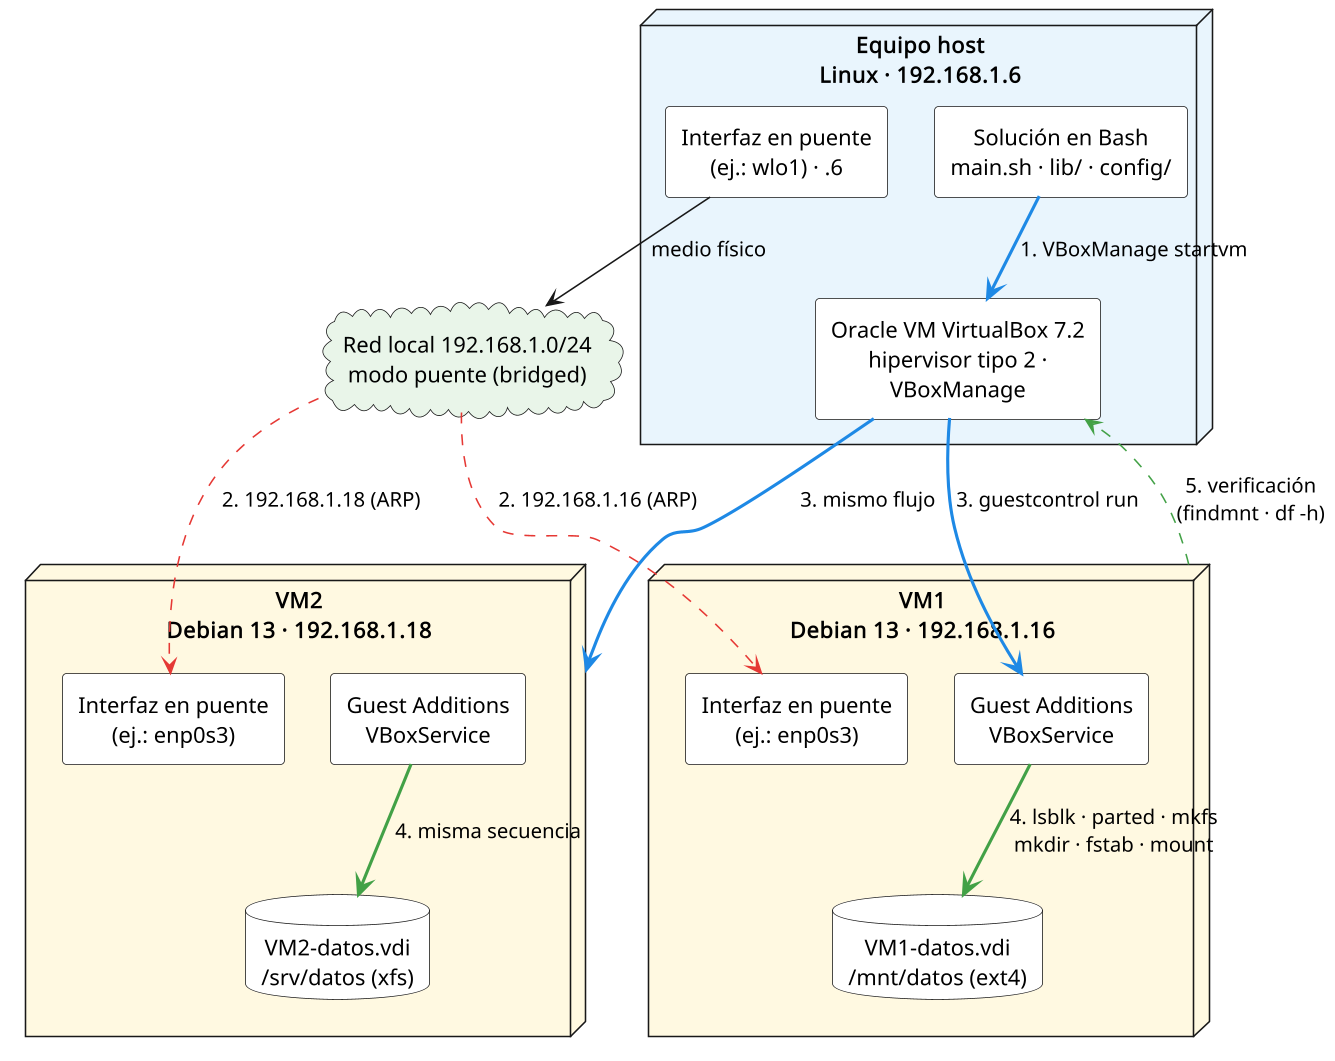
\includegraphics[width=0.95\textwidth]{escenario.png}
    \caption{Escenario de despliegue: \host{}, VirtualBox, red en modo puente, \vm{} y almacenamiento adicional}
    \label{fig:escenario}
\end{figure}

\subsection{Arquitectura y Comunicación entre Host y Guest}
\label{sub:arquitectura}

La solución se estructura en tres planos diferenciados. Un punto de entrada único, \texttt{main.sh}, recibe el nombre de la \vm{} objetivo, carga su archivo de configuración desde \texttt{config/} y coordina la ejecución; las bibliotecas de \texttt{lib/} concentran funciones reutilizables de orquestación, comunicación y almacenamiento; y los archivos de configuración por \vm{} declaran los parámetros que cambian entre máquinas: disco objetivo, punto de montaje, sistema de archivos y credenciales \parencite{bash_best_practices}. Con esta separación, el mismo algoritmo se aplica a \texttt{VM1} y \texttt{VM2} sin modificar el código, y las verificaciones con ShellCheck y BATS descritas en el Marco Teórico recaen sobre funciones pequeñas e independientes \parencite{shellcheck, bats_testing}. El lenguaje de implementación es Bash, justificado en la Subsección~\ref{sub:bash} por su disponibilidad nativa en el \host{} y por su acceso directo a la interfaz de línea de comandos \texttt{VBoxManage} \parencite{virtualbox_vboxmanage}.

La comunicación con el invitado se establece con la Guest Control API (\texttt{VBoxManage guestcontrol}), mecanismo que satisface el requerimiento de utilizar las \guestadditions{} para la interacción \parencite{virtualbox_guestcontrol}. En este mecanismo el \host{} entrega las órdenes al hipervisor, éste las transporta al servicio \texttt{VBoxService} en ejecución dentro de la \vm{} y el resultado regresa por el mismo canal; ese trayecto no atraviesa la red en puente, de modo que la ejecución de comandos no depende de conocer de antemano la dirección IP del invitado \parencite{virtualbox_guestadditions, virtualbox_advanced_topics}. La autenticación se realiza con un usuario y una contraseña del propio sistema invitado, leídos del archivo de configuración antes de abrir la sesión, de manera que ninguna etapa solicita credenciales, comandos ni pulsaciones al usuario \parencite{virtualbox_guestcontrol}.

La dirección IP de la \vm{} sí se identifica de forma automática, porque es un requisito del proceso y se emplea para verificar la conectividad y registrar la máquina atendida. El mecanismo principal consulta la propiedad que publican las \guestadditions{} en el hipervisor. La orden \texttt{VBoxManage guestproperty get VM1} lee la propiedad \path{/VirtualBox/GuestInfo/Net/0/V4/IP} y devuelve la dirección vigente, sin sondear la red ni exigir servicios adicionales en el invitado \parencite{virtualbox_guestadditions, virtualbox_vboxmanage}. Como respaldo, y en particular si la propiedad aún no se ha actualizado tras el arranque, la solución consulta la tabla ARP completa del \host{} con \texttt{ip neigh} y selecciona la entrada cuya dirección MAC coincide con la del adaptador de la \vm{} reportada por \texttt{VBoxManage showvminfo}, operación que no exige conocer el nombre de ninguna interfaz; si éste fuera necesario, se obtiene en tiempo de ejecución con \texttt{ip route get} a partir de la dirección recién identificada. Del mismo modo, la solución nunca utiliza el nombre de la interfaz del invitado, el cual ni la Guest Control ni la consulta de propiedades requieren. En ambos casos la dirección IP es un resultado que la solución obtiene, valida y registra, nunca un valor fijo codificado en el programa \parencite{virtualbox_networking}.

\subsection{Algoritmo de Automatización (Idempotente)}
\label{sub:algoritmo}

El algoritmo se organiza en tres etapas que se ejecutan de forma secuencial y sin intervención del usuario: una etapa de preparación en el \host{}, una etapa de preparación del almacenamiento que se despacha al invitado con \texttt{VBoxManage guestcontrol} y una etapa de verificación y cierre que vuelve a ejecutarse en el \host{}. La Figura~\ref{fig:algoritmo} resume ese flujo en un diagrama de procesos con dos carriles, lo que permite distinguir en cada nodo qué equipo ejecuta la acción.

En la etapa de preparación, el punto de entrada carga la configuración de la \vm{} objetivo, comprueba si está encendida y, de no estarlo, la enciende con \texttt{VBoxManage startvm} y aguarda la respuesta de \texttt{VBoxService}; después identifica su dirección IP en tiempo de ejecución, según se describió en la Subsección~\ref{sub:arquitectura}, y despacha las órdenes al invitado \parencite{virtualbox_guestcontrol, virtualbox_guestadditions}.

La etapa de almacenamiento es idempotente porque cada acción está precedida por una guarda que consulta el estado actual antes de modificarlo \parencite{idempotency_concept}. La primera guarda utiliza \texttt{lsblk} para identificar el disco adicional por su tamaño y comprobar si carece de tabla de particiones; solo en ese caso crea una tabla GPT con una partición mediante \texttt{parted} \parencite{linux_storage_management}. La segunda verifica, con \texttt{blkid}, si la partición ya contiene un sistema de archivos; de lo contrario ejecuta \texttt{mkfs.ext4} o \texttt{mkfs.xfs} según la configuración de la \vm{}. La tercera consulta \texttt{findmnt} y el contenido de \texttt{/etc/fstab} y, únicamente si el montaje no está declarado ni activo, obtiene el UUID, crea el punto de montaje con \texttt{mkdir -p}, añade la entrada por UUID para que el montaje persista entre reinicios y ejecuta \texttt{mount -a} \parencite{uuid_fstab, lsb_fhs}.

Finalmente, la etapa de verificación confirma con \texttt{findmnt} y \texttt{df -h} que el almacenamiento quedó montado y registra el resultado: la ejecución termina con código~0 cuando la verificación es correcta y con código~1 cuando alguna guarda o verificación falla, de modo que el estado inconsistente se detecta de inmediato \parencite{bash_best_practices}. Como consecuencia de las guardas, re-ejecutar la solución sobre una \vm{} ya configurada no reformatea el disco ni duplica entradas en \texttt{/etc/fstab} y deja intactos los datos persistidos; la misma secuencia aplicada a \texttt{VM1} y \texttt{VM2} cambia únicamente los parámetros de entrada \parencite{idempotency_concept, ansible_up_running}.

\begin{figure}[H]
    \centering
    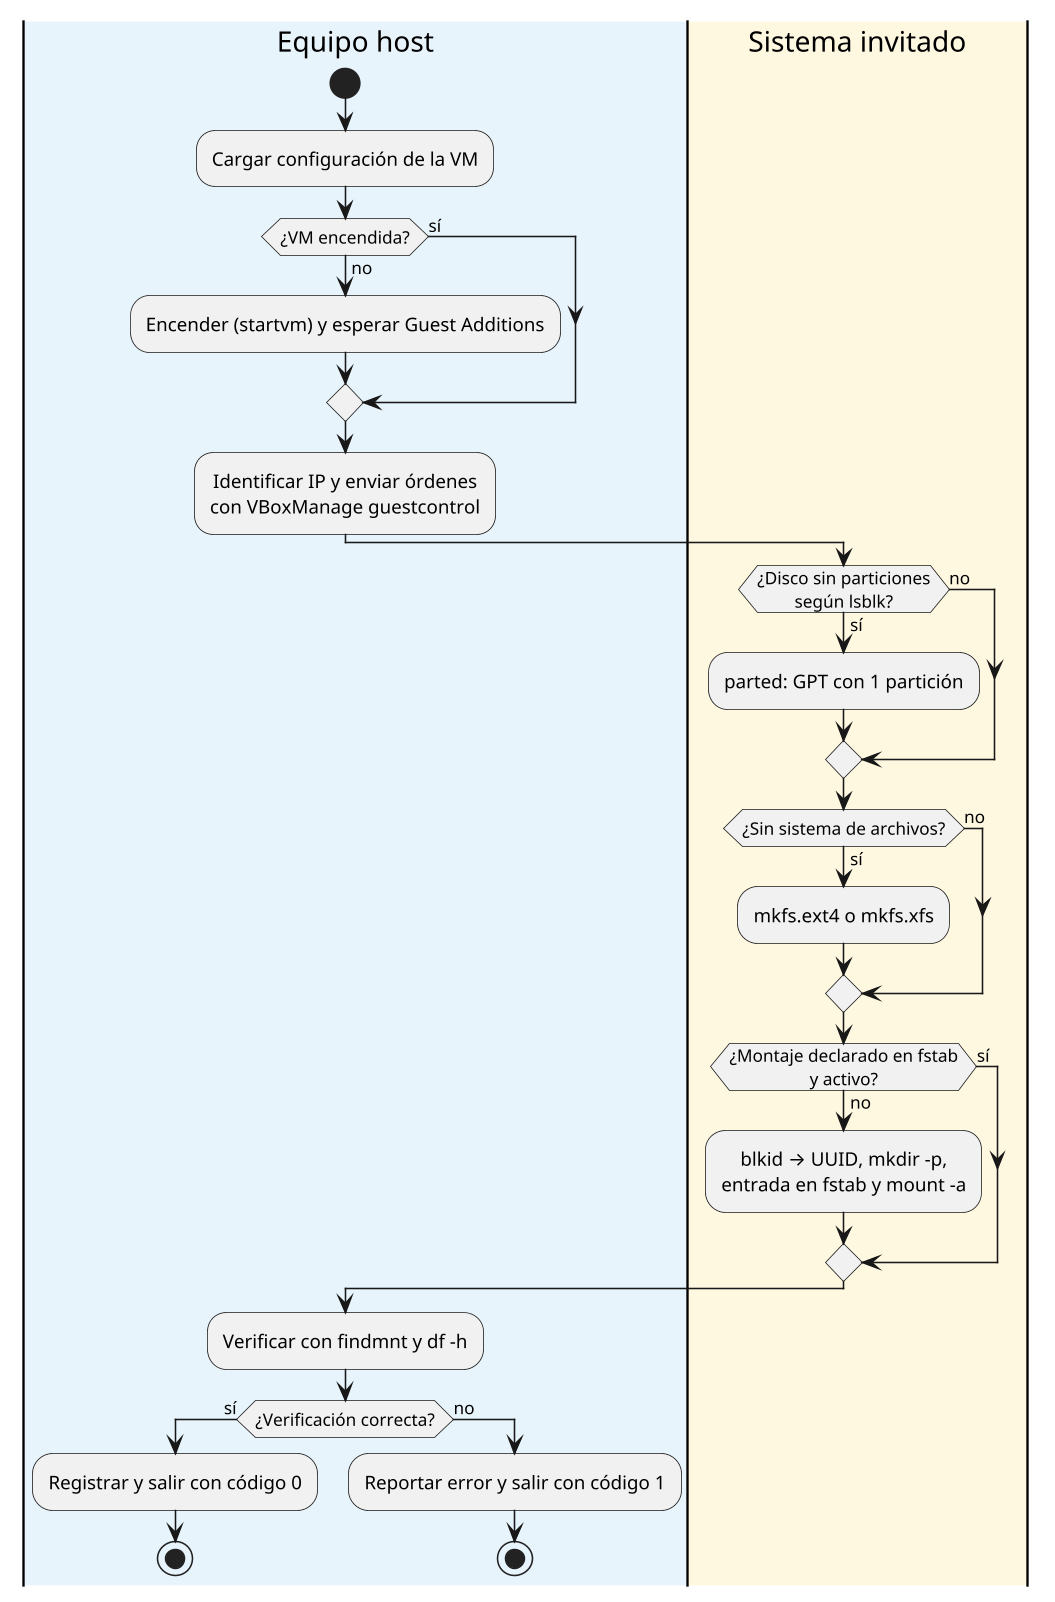
\includegraphics[width=0.7\textwidth]{algoritmo.png}
    \caption{Diagrama de procesos de la automatización idempotente, con las etapas ejecutadas en el \host{} y en el sistema invitado}
    \label{fig:algoritmo}
\end{figure}
% ==================== IMPLEMENTACIÓN ====================
\section{Implementación}

\subsection{Estructura del Código}
% TODO: Describir organización de archivos/scripts.
% Ejemplo:
% \begin{itemize}
%     \item \texttt{main.sh}: punto de entrada
%     \item \texttt{lib/common.sh}: funciones compartidas (logging, validación, ejecución remota)
%     \item \texttt{lib/storage.sh}: funciones de almacenamiento (particionar, formatear, montar, fstab)
%     \item \texttt{config/vm1.conf}, \texttt{config/vm2.conf}: parámetros por VM
% \end{itemize}
% Explicar criterio de modularidad y reutilización.

\subsection{Script / Programa Principal}
% TODO: Incluir fragmentos clave con \lstinputlisting.
% \lstinputlisting[caption={Script principal: detección de IP y orquestación}, label={lst:main}]{../scripts/main.sh}
% \lstinputlisting[caption={Funciones de almacenamiento idempotentes}, label={lst:storage}]{../scripts/lib/storage.sh}
%
% Explicar secciones clave:
% - Parseo de argumentos / lectura de configuración
% - Detección automática de IP de la VM
% - Establecimiento de comunicación (Guest Control o SSH)
% - Ejecución remota de comandos de preparación de almacenamiento
% - Verificaciones de idempotencia en cada paso
% - Manejo de salida y códigos de error

\subsection{Parametrización para Múltiples VMs}
% TODO: Explicar qué parámetros varían entre VMs y cómo se gestionan.
% Parámetros variables:
% - IP / hostname de la VM
% - Usuario para conexión (root o usuario con sudo)
% - Dispositivo de disco objetivo (ej. /dev/sdb, /dev/vdb)
% - Punto de montaje deseado (ej. /mnt/datos, /data)
% - Tipo de sistema de archivos (ext4, xfs)
% - Credenciales / clave SSH
%
% Estrategia: archivo de configuración por VM (INI, YAML, JSON, o .env) o variables de entorno.
% Ejemplo de archivo config:
% \begin{verbatim}
% VM_IP=192.168.1.50
% VM_USER=admin
% DISK_DEVICE=/dev/sdb
% MOUNT_POINT=/mnt/datos
% FS_TYPE=ext4
% \end{verbatim}

\subsection{Manejo de Errores y Casos Edge}
% TODO: Documentar estrategias de robustez.
% - Timeouts en conexión y comandos remotos
% - Reintentos con backoff (ej. esperar a que Guest Additions estén listas)
% - Validaciones previas: VM encendida, red accesible, disco existe, espacio suficiente
% - Códigos de salida significativos (0=ok, 1=error config, 2=error conexión, 3=error almacenamiento)
% - Logging estructurado (timestamp, nivel, mensaje) a archivo y stdout
% - Limpieza en caso de fallo parcial (no dejar sistema en estado inconsistente)

\subsection{Evidencias de Pruebas}
% TODO: Completar tabla con las 6 pruebas requeridas por el enunciado (punto 5).
% Para cada prueba: condición inicial, procedimiento, resultado esperado, resultado obtenido, evidencia.
%
% \begin{longtable}{@{}p{0.5cm}p{2.5cm}p{2.5cm}p{3cm}p{2.5cm}p{2.5cm}p{2.5cm}@{}}
% \toprule
% \textbf{ID} & \textbf{Prueba} & \textbf{Condición Inicial} & \textbf{Procedimiento} & \textbf{Resultado Esperado} & \textbf{Resultado Obtenido} & \textbf{Evidencia} \\
% \midrule
% \endhead
% 1 & Configuración inicial VM1 & VM1 sin disco configurado, encendida, Guest Additions OK & Ejecutar solución contra VM1 & Disco particionado, formateado, montado en /mnt/datos, entrada en fstab & [Pendiente] & Captura terminal / log \\
% 2 & Configuración inicial VM2 & VM2 sin disco configurado, encendida, Guest Additions OK & Ejecutar solución contra VM2 & Mismo resultado que VM1, parámetros distintos & [Pendiente] & Captura terminal / log \\
% 3 & Disponibilidad almacenamiento & Proceso completado en VM1 & \texttt{df -h}, \texttt{lsblk}, escribir archivo prueba & Almacenamiento accesible, escribible, con espacio esperado & [Pendiente] & Captura \texttt{df -h}, archivo creado \\
% 4 & Persistencia tras reboot & VM1 con almacenamiento configurado & Reiniciar VM1 (\texttt{reboot}), verificar montaje & Almacenamiento montado automáticamente tras reinicio & [Pendiente] & Captura \texttt{findmnt} post-reboot \\
% 5 & Re-ejecución en VM configurada & VM1 ya configurada (prueba 1) & Ejecutar solución nuevamente sobre VM1 & Sin pérdida de datos, sin reformatear, sin duplicar fstab, salida exitosa & [Pendiente] & Log ejecución, \texttt{blkid} sin cambios \\
% 6 & Condición de fallo & VM apagada / sin Guest Additions / disco inexistente & Ejecutar solución & Error controlado, mensaje claro, código salida ≠ 0, sin cambios en sistema & [Pendiente] & Captura error, log \\
% \bottomrule
% \caption{Resumen de pruebas ejecutadas y evidencias}
% \label{tab:pruebas}
% \end{longtable}
%
% Adjuntar evidencias como capturas de pantalla en \texttt{images/} y referenciarlas:
% \begin{figure}[H]
%     \centering
%     \includegraphics[width=0.8\textwidth]{evidencia_prueba1.png}
%     \caption{Evidencia prueba 1: configuración inicial VM1}
%     \label{fig:evidencia1}
% \end{figure}
% ==================== CONCLUSIONES ====================
\section{Conclusiones}

\subsection{Logros Alcanzados}

Se desarrolló una solución completa de automatización que prepara el almacenamiento adicional de una \vm{} GNU/Linux desde el \host{}, sin intervención manual alguna: la solución enciende la \vm{}, espera a que el sistema invitado esté disponible, identifica su dirección IP en tiempo de ejecución y ejecuta la secuencia de identificación del disco, particionado, creación del sistema de archivos, punto de montaje y montaje persistente en \texttt{/etc/fstab} \parencite{linux_storage_management, uuid_fstab}. La comunicación \host{}-\vm{} se materializa con la Guest Control API de VirtualBox, de modo que ninguna operación exige contraseñas, comandos interactivos ni pulsaciones de tecla durante la corrida \parencite{virtualbox_guestcontrol}.

El resultado es una orden única, \texttt{vboxdisk apply}, reproducible porque la misma configuración declarativa conduce al mismo estado final, y reutilizable porque la lógica no está ligada a una \vm{} concreta: el archivo \texttt{vdisk.yml} parametriza por máquina el usuario, el disco, el tamaño, el sistema de archivos y el punto de montaje, y la misma corrida convergió sobre \texttt{VM1} con ext4 en \texttt{/mnt/datos} y sobre \texttt{VM2} con xfs en \texttt{/srv/datos}. El algoritmo es idempotente: re-ejecutar la solución sobre una \vm{} ya configurada no reformatea el disco, no pierde los datos persistidos ni duplica entradas en \texttt{/etc/fstab}, porque cada acción destructiva está precedida de una guarda de solo lectura que contrasta el estado real con el declarado \parencite{idempotency_concept}.

\subsection{Cumplimiento de Requisitos del Parcial}

\begin{itemize}
    \item \textbf{Comunicación \host{}-\vm{} (3.1):} Guest Control API con obtención automática de la dirección IP a partir de la propiedad que publican las \guestadditions{} y respaldo sobre la tabla ARP, en red en modo puente \parencite{virtualbox_guestcontrol, virtualbox_networking}.
    \item \textbf{Automatización completa (3.2):} cero intervención manual; las credenciales se pasan mediante un fichero temporal que se destruye al terminar, tanto en el \host{} como en el invitado.
    \item \textbf{Preparación de almacenamiento (3.3):} particionado, creación del sistema de archivos, punto de montaje, entrada por UUID en \texttt{fstab} y montaje, ejecutados por el script invitado \texttt{guest\_ensure.sh} \parencite{kernel_block_devices, lsb_fhs}.
    \item \textbf{Ejecución repetida / idempotencia (3.4):} mecanismo descrito en la Subsección~\ref{sub:algoritmo} y comprobado en la prueba~5 de la Tabla~\ref{tab:pruebas}.
    \item \textbf{Aplicación a múltiples \vm{} (3.5):} probado con dos \vm{} cuya única diferencia son los valores de \texttt{vdisk.yml}; ninguna lógica del programa depende de una máquina particular.
    \item \textbf{Tiempo de ejecución (3.6):} medido con los dos cronómetros integrados; las mediciones de tres corridas se reportan en la Tabla~\ref{tab:tiempos}.
    \item \textbf{Tecnología (4):} Shell script (Bash) en un \host{} GNU/Linux, con \texttt{make} como sistema de construcción y ShellCheck y BATS como verificación \parencite{bash_best_practices, shellcheck, bats_testing}.
    \item \textbf{Pruebas (5):} seis pruebas diseñadas con condición inicial, procedimiento, resultado esperado, resultado obtenido y evidencia, en la Tabla~\ref{tab:pruebas}.
    \item \textbf{Escenario (6):} diagrama de despliegue y descripción en la Sección~\ref{sub:escenario}.
\end{itemize}

\subsection{Problemas Encontrados y su Solución}

El desarrollo presentó cuatro problemas que se resolvieron de la siguiente manera.

\begin{description}[style=nextline, leftmargin=1.2cm]
    \item[Código de salida ambiguo] La llamada \texttt{VBoxManage guestcontrol run} devuelve códigos que mezclan los del proceso invitado con los del propio servicio Guest Control, de modo que un fallo del servicio y un código de salida del script no eran distinguibles en el \host{}. Se resolvió con una línea centinela \texttt{VBOXDISK\_EXIT=<n>} emitida por el script invitado sobre su salida estándar: el \host{} la interpreta de forma explícita y solo asigna el código~0 cuando la centinela indica convergencia correcta.
    \item[Limpieza de credenciales] La trampa de salida del \host{} destruía primero los ficheros temporales de contraseña locales, pero el script invitado aún necesitaba el suyo para terminar de eliminarse a sí mismo en el invitado. Se reordenó la secuencia: primero se limpian los directorios temporales del invitado con Guest Control y solo después se revuelven los ficheros del \host{}, de modo que ninguna corrida, ni siquiera una interrumpida, deja credenciales en ninguno de los dos lados.
    \item[Nombres de \vm{} con guion] Las consultas a \texttt{yq} construían las rutas de acceso como \texttt{VM1.mount\_point}, lo que interpretaba mal los nombres con guion. Se pasan las claves siempre entre comillas (\texttt{."\$\{vm\}".\"\$\{key\}\"}), de modo que cualquier nombre que supere la validación se lee correctamente.
    \item[Restricciones de Guest Control] El servicio no admite la eliminación recursiva de directorios con \texttt{guestcontrol rm} y \texttt{mktemp} anuncia el directorio creado con un prefijo de texto. Se eliminan los directorios temporales con \texttt{guestcontrol run -- /bin/rm -rf} y se extrae la ruta con el prefijo indicado en la documentación de la utilidad \parencite{virtualbox_guestcontrol}.
\end{description}

\subsection{Herramientas de Inteligencia Artificial Utilizadas}

Se empleó un agente de inteligencia artificial basado en un modelo de lenguaje, integrado en la terminal, para las siguientes tareas. En primer lugar, como asistente de desarrollo: diseño del enfoque declarativo y del algoritmo de cinco etapas, generación del código Bash de las bibliotecas en \texttt{src/}, del \texttt{Makefile}, de los ficheros de prueba BATS y del doble de \texttt{VBoxManage}. En segundo lugar, como verificador documental: se consultó la documentación oficial y el código fuente de VirtualBox para confirmar el comportamiento exacto de \texttt{guestcontrol run}, \texttt{mktemp}, \texttt{copyto} y \texttt{rm}, lo que permitió detectar que \texttt{rm} no admite eliminación recursiva y corregir el diseño de la limpieza del invitado antes de ejecutarlo. En tercer lugar, como redactor y corrector: redacción de las secciones del presente documento en \LaTeX{}, seguimiento de las convenciones del trabajo y corrección mecánica de los hallazgos de ShellCheck y de las advertencias de sobreancho de la composición tipográfica. La ejecución de las pruebas contra las \vm{} reales y la validación final de los resultados corresponden a los autores del trabajo.

\subsection{Limitaciones Identificadas}

La solución exige que las \guestadditions{} estén instaladas y funcionando en el invitado, pues tanto la espera de disponibilidad como la obtención de la dirección IP dependen de ellas \parencite{virtualbox_guestadditions}. Supone además una red en modo puente accesible desde el \host{} y un único disco adicional vacío por \vm{}: no aborda LVM, varios discos ni discos con contenido previo que deba conservarse. Las credenciales de las \vm{} viven en \texttt{vdisk.yml} o en un fichero legible por el usuario, suficiente para un entorno de pruebas pero no para uno productivo, donde convendría un almacén de secretos.

\subsection{Trabajo Futuro}

Extensiones naturales incluyen el soporte de LVM y de varios discos por \vm{}, la ejecución desde un pipeline de integración continua, la traslación de la misma idea declarativa a otras plataformas de virtualización y la sustitución de la autenticación por contraseña por claves de \texttt{ssh} cuando el entorno lo permita. En el plano operativo, la inclusión de métricas y de una bitácora estructurada facilitaría la observabilidad de corridas sobre muchas \vm{} simultáneas \parencite{ansible_up_running}.


% ==================== BIBLIOGRAFÍA ====================
\newpage
\printbibliography

\end{document}
